%\documentclass[prd,twocolumn,aps,psfig,showpacs,nofootinbib,nobibnotes,superscriptaddress,preprintnumbers,times]{revtex4}
\documentclass[prd,twocolumn,aps,psfig,nofootinbib,nobibnotes,superscriptaddress,preprintnumbers,times]{revtex4-2}
\setlength{\topmargin}{-14mm}
\usepackage{graphicx,bm,color,amsmath,amssymb, mathtools,subcaption}
\graphicspath{{./fig/}}

\usepackage[hidelinks]{hyperref}
\hypersetup{
  colorlinks   = true, %Colours links instead of ugly boxes
  urlcolor     = blue, %Colour for external hyperlinks
  linkcolor    = red, %Colour of internal links
  citecolor    = blue %Colour of citations
}

\def\red{\textcolor{red}}
\def\blue{\textcolor{blue}}

%|||||||||||||||||||||||||||||||||||||||||||||||||||||||||||||||||||
%             Customized Commands
%|||||||||||||||||||||||||||||||||||||||||||||||||||||||||||||||||||
%  mathematical abbreviations
%
%
%
\newcommand{\BoldVec}[1]{\mathchoice%
  {\mbox{\boldmath $\displaystyle     #1$}}%
  {\mbox{\boldmath $\textstyle        #1$}}%
  {\mbox{\boldmath $\scriptstyle      #1$}}%
  {\mbox{\boldmath $\scriptscriptstyle#1$}}%
}
%\newcommand{\BoldVec}[1]{\bm{#1}}}
%
% math debs
\newcommand{\EQ}{\begin{equation}}
\newcommand{\EN}{\end{equation}}
\newcommand{\EQA}{\begin{eqnarray}}
\newcommand{\ENA}{\end{eqnarray}}
\newcommand{\eq}[1]{(\ref{#1})}
\newcommand{\EEq}[1]{Equation~(\ref{#1})}
\newcommand{\Eq}[1]{Eq.~(\ref{#1})}
\newcommand{\Eqs}[2]{Eqs~(\ref{#1}) and~(\ref{#2})}
\newcommand{\EEqs}[2]{Equations~(\ref{#1}) and~(\ref{#2})}
\newcommand{\eqs}[2]{(\ref{#1}) and~(\ref{#2})}
\newcommand{\Eqss}[2]{Eqs~(\ref{#1})--(\ref{#2})}
%\newcommand{\Sec}[1]{\S\,\ref{#1}}
%\newcommand{\Secs}[2]{\S\S\,\ref{#1} and~\ref{#2}}
\newcommand{\Sec}[1]{Sec.~\ref{#1}}
\newcommand{\Secs}[2]{Secs.~\ref{#1} and~\ref{#2}}
\newcommand{\App}[1]{Appendix~\ref{#1}}
\newcommand{\Fig}[1]{Fig.~\ref{#1}}
\newcommand{\FFig}[1]{Figure~\ref{#1}}
\newcommand{\Tab}[1]{Table~\ref{#1}}
\newcommand{\Figs}[2]{Figs.~\ref{#1} and \ref{#2}}
\newcommand{\Tabs}[2]{Tables~\ref{#1} and \ref{#2}}
%\newcommand{\bra}[1]{\langle #1\rangle}
\newcommand{\bbra}[1]{\left\langle #1\right\rangle}
\newcommand{\mean}[1]{\overline #1}
\newcommand{\meanB}{\overline{B}}
\newcommand{\meanC}{\overline{C}}
\newcommand{\meanU}{\overline{U}}
\newcommand{\meanW}{\overline{W}}
\newcommand{\meanPhi}{\overline{\Phi}}
\newcommand{\meanF}{\overline{\cal F}}
\newcommand{\meanR}{\overline{\cal R}}
\newcommand{\meanAA}{\overline{\bm{A}}}
\newcommand{\meanBB}{\overline{\bm{B}}}
\newcommand{\meanEE}{\overline{\bm{E}}}
\newcommand{\meanUU}{\overline{\bm{U}}}
\newcommand{\meanWW}{\overline{\bm{W}}}
\newcommand{\meanJJ}{\overline{\mbox{\boldmath $J$}}}
\newcommand{\meanuu}{\overline{\mbox{\boldmath $u$}}}
\newcommand{\meanGG}{\overline{\mbox{\boldmath $G$}}}
\newcommand{\meanAB}{\overline{\mbox{\boldmath $A\cdot B$}}}
\newcommand{\meanAoBo}{\overline{\mbox{\boldmath $A_0\cdot B_0$}}}
\newcommand{\meanApoBpo}{\overline{\mbox{\boldmath $A'_0\cdot B'_0$}}}
\newcommand{\meanApBp}{\overline{\mbox{\boldmath $A'\cdot B'$}}}
\newcommand{\meanuxB}{\overline{\mbox{\boldmath $\delta u\times \delta B$}}}
\newcommand{\meanemfs}{\overline{\cal E} {}}
\newcommand{\meanemf}{\overline{\mbox{\boldmath ${\cal E}$}} {}} %redundant
\newcommand{\meanAAAA}{\overline{\mbox{\boldmath ${\mathsf A}$}} {}}
\newcommand{\meanSSSS}{\overline{\mbox{\boldmath ${\mathsf S}$}} {}}
\newcommand{\meanAAA}{\overline{\mathsf{A}}}
\newcommand{\meanSSS}{\overline{\mathsf{S}}}
\newcommand{\meanCC}{\overline{\mbox{\boldmath ${\cal C}$}} {}}
\newcommand{\meanFF}{\overline{\mbox{\boldmath ${\cal F}$}} {}}
\newcommand{\meanRR}{\overline{\mbox{\boldmath ${\cal R}$}} {}}
\newcommand{\calFF}{\overline{\mbox{\boldmath ${\cal F}$}} {}}
\newcommand{\meanEMF}{\overline{\mbox{\boldmath ${\cal E}$}} {}}
\newcommand{\tildeFFFF}{\tilde{\mbox{\boldmath ${\cal F}$}}{}}{}
\newcommand{\hatFFFF}{\hat{\mbox{\boldmath ${\cal F}$}}{}}{}
\newcommand{\meanFFFF}{\overline{\mbox{\boldmath ${\cal F}$}}{}}{}
\newcommand{\meanFFF}{\overline{\cal F}}
\newcommand{\hatOO}{\hat{\bm{\Omega}}}
\newcommand{\hatAA}{\hat{\bm{A}}}
\newcommand{\hatBB}{\hat{\bm{B}}}
\newcommand{\tildeh}{\tilde{h}}
\newcommand{\tildeT}{\tilde{T}}
\newcommand{\tildehhh}{\tilde{\sf h}}
\newcommand{\tildeTTT}{\tilde{\sf T}}
%
% tilde
%
\newcommand{\eee}{{\sf e}}
\newcommand{\hhh}{{\sf h}}
\newcommand{\TTT}{{\sf T}}
\newcommand{\tildexx}{\tilde{\bm{x}}}
\newcommand{\tildeBB}{\tilde{\bm{B}}}
\newcommand{\tildeJJ}{\tilde{\bm{J}}}
\newcommand{\tildeA}{\tilde{A}}
\newcommand{\tildeB}{\tilde{B}}
\newcommand{\tildeJ}{\tilde{J}}
\newcommand{\tildeemf}{\tilde{\cal E}}
\newcommand{\teps}{\tilde{\epsilon} {}}
\newcommand{\tkapz}{\tilde{\kappa_0}}
\newcommand{\Oh}{\hat{\Omega}}
\newcommand{\zh}{\hat{z}}
\newcommand{\PC}{{\sc Pencil Code}~}
\newcommand{\PCS}{{\sc Pencil Code}}
%
%  unit vectors
%
\newcommand{\nullvector}{{\bf0}}
\newcommand{\nnn}{\hat{\mbox{\boldmath $n$}} {}}
\newcommand{\vvv}{\hat{\mbox{\boldmath $v$}} {}}
\newcommand{\rr}{\hat{\mbox{\boldmath $r$}} {}}
\newcommand{\xxx}{\hat{\mbox{\boldmath $x$}} {}}
\newcommand{\yyy}{\hat{\mbox{\boldmath $y$}} {}}
\newcommand{\zz}{\hat{\mbox{\boldmath $z$}} {}}
\newcommand{\pp}{\hat{\mbox{\boldmath $\phi$}} {}}
\newcommand{\ttt}{\hat{\mbox{\boldmath $\theta$}} {}}
\newcommand{\OOO}{\hat{\mbox{\boldmath $\Omega$}} {}}
\newcommand{\ooo}{\hat{\mbox{\boldmath $\omega$}} {}}
\newcommand{\BBBB}{\hat{\mbox{\boldmath $B$}} {}}
\newcommand{\kunit}{\hat{\mbox{$k$}} {}}
\newcommand{\nunit}{\hat{\mbox{$n$}} {}}
%
%  hatted quantities
%
\newcommand{\hatU}{\hat{U}}
\newcommand{\hatUU}{\hat{\bm{U}}}
%
%  vectors
%
\newcommand{\gggg}{\BoldVec{g} {}}
\newcommand{\ddd}{\BoldVec{d} {}}
\newcommand{\rrr}{\BoldVec{r} {}}
\newcommand{\xx}{\BoldVec{x}{}}
\newcommand{\yy}{\BoldVec{y} {}}
\newcommand{\zzz}{\BoldVec{z} {}}
\newcommand{\uu}{\BoldVec{u} {}}
\newcommand{\vv}{\BoldVec{v} {}}
\newcommand{\ww}{\BoldVec{w} {}}
\newcommand{\mm}{\BoldVec{m} {}}
\newcommand{\PP}{\BoldVec{P} {}}
\newcommand{\QQ}{\BoldVec{Q} {}}
\newcommand{\RR}{\BoldVec{R} {}}
\newcommand{\UU}{\BoldVec{U} {}}
\newcommand{\bb}{\BoldVec{b} {}}
\newcommand{\qq}{\BoldVec{q} {}}
\newcommand{\BB}{\BoldVec{B} {}}
\newcommand{\HH}{\BoldVec{H} {}}
\newcommand{\II}{\BoldVec{I} {}}
\newcommand{\AAA}{\BoldVec{A} {}}
\newcommand{\aaa}{\BoldVec{a} {}}
\newcommand{\aaaa}{\BoldVec{a} {}} %(convert aaa -> aaaa, compatibility problem)
%\newcommand{\eee}{\BoldVec{e} {}}
\newcommand{\jj}{\BoldVec{j} {}}
\newcommand{\JJ}{\BoldVec{J} {}}
\newcommand{\nn}{\BoldVec{n} {}}
\newcommand{\ee}{\BoldVec{e} {}}
\newcommand{\ff}{\BoldVec{f} {}}
\newcommand{\hh}{\BoldVec{h} {}}
\newcommand{\EE}{\BoldVec{E} {}}
\newcommand{\FF}{\BoldVec{F} {}}
\newcommand{\TT}{\BoldVec{T} {}}
\newcommand{\CC}{\BoldVec{C} {}}
\newcommand{\KK}{\BoldVec{K} {}}
\newcommand{\MM}{\BoldVec{M} {}}
\newcommand{\GG}{\BoldVec{G} {}}
\newcommand{\kk}{\BoldVec{k} {}}
\newcommand{\SSS}{\BoldVec{S} {}}
\newcommand{\grav}{\BoldVec{g} {}}
\newcommand{\nab}{\BoldVec{\nabla} {}}
\newcommand{\OO}{\BoldVec{\Omega} {}}
\newcommand{\oo}{\BoldVec{\omega} {}}
\newcommand{\LL}{\BoldVec{\Lambda} {}}
\newcommand{\llambda}{\BoldVec{\lambda} {}}
\newcommand{\pomega}{\BoldVec{\varpi} {}}
%
%  correlation tensors
%
\newcommand{\RRRR}{\bm{\mathsf{R}}}
\newcommand{\SSSS}{\bm{\mathsf{S}}}
\newcommand{\LLLL}{\mbox{\boldmath ${\sf L}$} {}}
\newcommand{\MMMM}{\bm{\mathsf{M}}}
\newcommand{\BBB}{\mbox{\boldmath ${\cal B}$} {}}
\newcommand{\emf}{\mbox{\boldmath ${\cal E}$} {}}
\newcommand{\FFF}{\mbox{\boldmath ${\cal F}$} {}}
\newcommand{\GGG}{\mbox{\boldmath ${\cal G}$} {}}
\newcommand{\HHH}{\mbox{\boldmath ${\cal H}$} {}}
\newcommand{\QQQ}{\mbox{\boldmath ${\cal Q}$} {}}
%
%  operators  (roman)
%
\newcommand{\ii}{{\rm i}}
\newcommand{\grad}{{\rm grad} \, {}}
\newcommand{\curl}{{\rm curl} \, {}}
\newcommand{\dive}{{\rm div}  \, {}}
\newcommand{\Dive}{{\rm Div}  \, {}}
\newcommand{\diag}{{\rm diag}  \, {}}
\newcommand{\DD}{{\rm D} {}}
\newcommand{\dd}{{\rm d} {}}
\newcommand{\const}{{\rm const}  {}}
\newcommand{\crit}{{\rm crit}  {}}
\def\degr{\hbox{$^\circ$}}
\def\la{\mathrel{\mathchoice {\vcenter{\offinterlineskip\halign{\hfil
$\displaystyle##$\hfil\cr<\cr\sim\cr}}}
{\vcenter{\offinterlineskip\halign{\hfil$\textstyle##$\hfil\cr<\cr\sim\cr}}}
{\vcenter{\offinterlineskip\halign{\hfil$\scriptstyle##$\hfil\cr<\cr\sim\cr}}}
{\vcenter{\offinterlineskip\halign{\hfil$\scriptscriptstyle##$\hfil\cr<\cr\sim\cr}}}}}
\def\ga{\mathrel{\mathchoice {\vcenter{\offinterlineskip\halign{\hfil
$\displaystyle##$\hfil\cr>\cr\sim\cr}}}
{\vcenter{\offinterlineskip\halign{\hfil$\textstyle##$\hfil\cr>\cr\sim\cr}}}
{\vcenter{\offinterlineskip\halign{\hfil$\scriptstyle##$\hfil\cr>\cr\sim\cr}}}
{\vcenter{\offinterlineskip\halign{\hfil$\scriptscriptstyle##$\hfil\cr>\cr\sim\cr}}}}}
%
%  numbers
%
\def\Ta{\mbox{\rm Ta}}
\def\Ra{\mbox{\rm Ra}}
\def\Ma{\mbox{\rm Ma}}
\def\Sh{\mbox{\rm Sh}}
\def\Roo{\mbox{\rm Ro}^{-1}}
\def\Pra{\mbox{\rm Pr}}
\def\Pran{\mbox{\rm Pr}}
\def\Pm{\mbox{\rm Pr}_{\rm M}}
\def\Rm{\mbox{\rm Re}_{\rm M}}
\def\Rey{\mbox{\rm Re}}
\def\Imag{\mbox{\rm Im}}
\def\Pe{\mbox{\rm Pe}}
\def\epsK{\epsilon_{\rm K}}
\def\epsM{\epsilon_{\rm M}}
\def\EEi{{\cal E}_i}
\def\EEK{{\cal E}_{\rm K}}
\def\EEM{{\cal E}_{\rm M}}
\def\EEKM{{\cal E}_{\rm K/M}}
\def\EEGW{{\cal E}_{\rm GW}}
\def\OmK{{\Omega}_{\rm K}}
\def\OmM{{\Omega}_{\rm M}}
\def\OmGW{{\Omega}_{\rm GW}}
\def\hrms{{h}_{\rm rms}}
\def\EEtot{{\cal E}_{\rm tot}}
\def\EErad{{\cal E}_{\rm rad}}
\def\EElam{{\cal E}_\lambda}
\def\EEcrit{{\cal E}_{\rm crit}}
\def\HHGW{{\cal H}_{\rm GW}}
\def\HHK{{\cal H}_{\rm K}}
\def\HHM{{\cal H}_{\rm M}}
\def\EGW{E_{\rm GW}}
\def\HGW{H_{\rm GW}}
\def\EK{E_{\rm K}}
\def\EM{E_{\rm M}}
\def\HM{H_{\rm M}}
\def\hc{h_{\rm c}}
\def\cs{c_{\rm s}}
\def\xiM{\xi_{\rm M}}
\def\xiK{\xi_{\rm K}}
\def\kf{k_{\rm f}}
%\def\kf{k_\ast}
\def\vA{v_{\rm A}}
\def\urms{u_{\rm rms}}
\def\Urms{U_{\rm rms}}
\def\Brms{B_{\rm rms}}
\def\kappaOO{\kappa_{\Omega\Omega}}
\def\kappaO{\kappa_{\Omega}}
\def\kappat{\kappa_{\rm t}}
\def\kappatz{\kappa_{\rm t0}}
\def\nut{\nu_{\rm t}}
\def\etatz{\eta_{\rm t0}}
\def\etat{\eta_{\rm t}}
\def\etaT{\eta_{\rm T}}
\def\Beq{B_{\rm eq}}
\def\tmax{t_{\max}}
%
\newcommand{\ea}{{\em et al. }}
\newcommand{\eaa}{{\em et al. }}
\def\half{{\textstyle{1\over2}}}
\def\threehalf{{\textstyle{3\over2}}}
\def\onethird{{\textstyle{1\over3}}}
\def\twothird{{\textstyle{2\over3}}}
\def\fourthird{{\textstyle{4\over3}}}
\def\quarter{{\textstyle{1\over4}}}
%
\newcommand{\W}{\,{\rm W}}
\newcommand{\V}{\,{\rm V}}
\newcommand{\kV}{\,{\rm kV}}
\newcommand{\MeV}{\,{\rm MeV}}
\newcommand{\GeV}{\,{\rm GeV}}
\newcommand{\T}{\,{\rm T}}
\newcommand{\uG}{\,\mu{\rm G}}
\newcommand{\G}{\,{\rm G}}
\newcommand{\Hz}{\,{\rm Hz}}
\newcommand{\mHz}{\,{\rm mHz}}
\newcommand{\nHz}{\,{\rm nHz}}
\newcommand{\uHz}{\,\mu{\rm Hz}}
\newcommand{\kHz}{\,{\rm kHz}}
\newcommand{\kG}{\,{\rm kG}}
\newcommand{\K}{\,{\rm K}}
\newcommand{\g}{\,{\rm g}}
\newcommand{\s}{\,{\rm s}}
\newcommand{\ms}{\,{\rm ms}}
\newcommand{\cm}{\,{\rm cm}}
\newcommand{\m}{\,{\rm m}}
\newcommand{\km}{\,{\rm km}}
\newcommand{\kms}{\,{\rm km/s}}
\newcommand{\kg}{\,{\rm kg}}
\newcommand{\Mm}{\,{\rm Mm}}
\newcommand{\pc}{\,{\rm pc}}
\newcommand{\kpc}{\,{\rm kpc}}
\newcommand{\Mpc}{\,{\rm Mpc}}
\newcommand{\yr}{\,{\rm yr}}
\newcommand{\Myr}{\,{\rm Myr}}
\newcommand{\Gyr}{\,{\rm Gyr}}
\newcommand{\erg}{\,{\rm erg}}
\newcommand{\mol}{\,{\rm mol}}
\newcommand{\dyn}{\,{\rm dyn}}
\newcommand{\J}{\,{\rm J}}
\newcommand{\RM}{\,{\rm RM}}
\newcommand{\AU}{\,{\rm AU}}
\newcommand{\A}{\,{\rm A}}
%
\def\hX{h_\times}
\def\hT{h_+}
\def\thT{\tilde{h}_+}
\def\thX{\tilde{h}_\times}
\def\dhT{\dot{h}_+}
\def\dhX{\dot{h}_\times}
\def\dhhT{\dot{\hat{h}}_+}
\def\dhhX{\dot{\hat{h}}_\times}
\def\dhhTX{\dot{\hat{h}}_{+/\times}}
\def\dthT{\dot{\tilde{h}}_+}
\def\dthX{\dot{\tilde{h}}_\times}
\def\dthTX{\dot{\tilde{h}}_{+/\times}}
%
%  journals
%
\newcommand{\arXiv}[3]{, ``#3,'' arXiv:#2 (#1).}
\newcommand{\yjcap}[3]{, J.\ Cosmol.\ Astropart.\ Phys. {\bf #2} (#1) #3.}
\newcommand{\yjas}[3]{, J. Atmosph. Sci. {\bf #2}, #3 (#1).}
\newcommand{\yan}[3]{, Astron. Nachr. {\bf #2}, #3 (#1).}
\newcommand{\yact}[3]{, Acta Astron. {\bf #2}, #3 (#1).}
\newcommand{\yana}[3]{, Astron. Astrophys. {\bf #2}, #3 (#1).}
\newcommand{\yanas}[3]{, Astron. Astrophys. Suppl. {\bf #2}, #3 (#1).}
\newcommand{\yanal}[3]{, Astron. Astrophys. Lett. {\bf #2}, #3 (#1).}
\newcommand{\yass}[3]{, Astrophys. Spa. Sci. {\bf #2}, #3 (#1).}
\newcommand{\ysci}[3]{, Science {\bf #2}, #3 (#1).}
\newcommand{\ysph}[3]{, Solar Phys. {\bf #2}, #3 (#1).}
\newcommand{\yjetp}[3]{, Sov. Phys. JETP {\bf #2}, #3 (#1).}
\newcommand{\yspd}[3]{, Sov. Phys. Dokl. {\bf #2}, #3 (#1).}
\newcommand{\ysov}[3]{, Sov. Astron. {\bf #2}, #3 (#1).}
\newcommand{\ysovl}[3]{, Sov. Astron. Lett. {\bf #2}, #3 (#1).}
\newcommand{\ymn}[3]{, Mon.\ Not.\ R.\ Astron.\ Soc.\ {\bf #2}, #3 (#1).}
\newcommand{\ymhd}[3]{, Magnetohydrohydrodyn. {\bf #2}, #3 (#1).}
\newcommand{\yqjras}[3]{, Quart. J. Roy. Astron. Soc. {\bf #2}, #3 (#1).}
\newcommand{\ynat}[3]{, Nature {\bf #2}, #3 (#1).}
\newcommand{\yjfm}[4]{, ``#4,'' J. Fluid Mech. {\bf #2}, #3 (#1).}
\newcommand{\pjfm}[1]{, J. Fluid Mech., in press (#1).}
\newcommand{\sjfm}[1]{, J. Fluid Mech., submitted (#1).}
\newcommand{\ypr}[3]{, Phys.\ Rev.\ {\bf #2}, #3 (#1).}
\newcommand{\yprd}[4]{, ``#4,'' Phys.\ Rev.\ D {\bf #2}, #3 (#1).}
\newcommand{\ypre}[3]{, Phys.\ Rev.\ E {\bf #2}, #3 (#1).}
\newcommand{\yprf}[4]{, ``#4,'' Phys.\ Rev.\ Fluids {\bf #2}, #3 (#1).}
\newcommand{\yprl}[4]{, ``#4,'' Phys.\ Rev.\ Lett.\ {\bf #2}, #3 (#1).}
\newcommand{\yphl}[3]{, Phys.\ Lett.\ {\bf #2}, #3 (#1).}
\newcommand{\pprl}[1]{, Phys. Rev. Lett., in press (#1).}
\newcommand{\yepl}[3]{, Europhys. Lett. {\bf #2}, #3 (#1).}
\newcommand{\pcsf}[2]{, Chaos, Solitons \& Fractals, in press (#1).}
\newcommand{\ycsf}[3]{, Chaos, Solitons \& Fractals{\bf #2}, #3 (#1).}
\newcommand{\yprs}[3]{, Proc. Roy. Soc. Lond. {\bf #2}, #3 (#1).}
\newcommand{\yptrs}[3]{, Phil. Trans. Roy. Soc. {\bf #2}, #3 (#1).}
\newcommand{\yptrsa}[4]{, ``#4,'' Phil. Trans. Roy. Soc. Lond. A, {\bf #2}, #3 (#1).}
\newcommand{\yjcp}[3]{, J. Comp. Phys. {\bf #2}, #3 (#1).}
\newcommand{\yjgr}[3]{, J. Geophys. Res. {\bf #2}, #3 (#1).}
\newcommand{\ygrl}[3]{, Geophys. Res. Lett. {\bf #2}, #3 (#1).}
\newcommand{\yobs}[3]{, Observatory {\bf #2}, #3 (#1).}
\newcommand{\yaj}[3]{, Astronom. J. {\bf #2}, #3 (#1).}
\newcommand{\sapj}[3]{, ``#3,'' Astrophys. J., submitted, arXiv:#2  (#1).}
\newcommand{\papj}[3]{, ``#3,'' Astrophys. J., in press, arXiv:#2  (#1).}
\newcommand{\yapj}[4]{, ``#4,'' Astrophys. J. {\bf #2}, #3 (#1).}
\newcommand{\yapjs}[3]{, Astrophys. J. Suppl. {\bf #2}, #3 (#1).}
\newcommand{\yapjl}[3]{, Astrophys. J. {\bf #2}, #3 (#1).}
\newcommand{\ycqg}[3]{, Class. Quant. Grav. {\bf #2}, #3 (#1).}
\newcommand{\ypp}[3]{, Phys. Plasmas {\bf #2}, #3 (#1).}
\newcommand{\yppcf}[3]{, Plasmas Phys. Contr. Fusion {\bf #2}, #3 (#1).}
\newcommand{\ppp}[1]{, Phys. Plasmas, in press (#1).}
\newcommand{\ypasj}[3]{, Publ. Astron. Soc. Japan {\bf #2}, #3 (#1).}
\newcommand{\ypac}[3]{, Publ. Astron. Soc. Pacific {\bf #2}, #3 (#1).}
\newcommand{\yaraa}[3]{, Ann. Rev. Astron. Astrophys. {\bf #2}, #3 (#1).}
\newcommand{\yanar}[3]{, Astron. Astrophys. Rev. {\bf #2}, #3 (#1).}
\newcommand{\yanp}[3]{, Ann. Phys. {\bf #2}, #3 (#1).}
\newcommand{\yanf}[3]{, Ann. Rev. Fluid Dyn. {\bf #2}, #3 (#1).}
\newcommand{\ypf}[4]{, ``#4,'' Phys. Fluids {\bf #2}, #3 (#1).}
\newcommand{\yphy}[3]{, Physica {\bf #2}, #3 (#1).}
\newcommand{\ygafd}[4]{, ``#4,'' Geophys. Astrophys. Fluid Dyn. {\bf #2}, #3 (#1).}
\newcommand{\yrpp}[3]{, Rep. Prog. Phys. {\bf #2}, #3 (#1).}
\newcommand{\yptp}[3]{, Progr. Theor. Phys. {\bf #2}, #3 (#1).}
\newcommand{\yjour}[5]{, ``#5,'' #2 {\bf #3}, #4 (#1).}
\newcommand{\pjour}[3]{, #2, in press (#1).}
\newcommand{\sjour}[3]{, #2, submitted (#1).}
\newcommand{\yprep}[2]{, #2, preprint (#1).}
\newcommand{\pproc}[3]{, (ed. #3), #2 (#1) (to appear).}
\newcommand{\yproc}[4]{, (ed. #4), pp. #2. #3 (#1).}
\newcommand{\ybook}[3]{, {\em #2}. #3 (#1).}
\newcommand{\neff}{N_{\rm eff}}
\newcommand{\dneff}{\Delta N_{\rm eff}}
\newcommand{\neffv}{N_{\rm eff}^{(\nu)}}

\newcommand{\inv}{\rm inv}

\usepackage{braket}

\begin{document}

\title{Stochastic Gravitational Wave Background Detection through NANOGrav 15-year Data Set in the View of Massive Gravity}

\date{\today}
\author{Chris~Choi}
\email{minyeonc@andrew.cmu.edu}
\affiliation{Department of Physics, Carnegie Mellon University, Pittsburgh, PA 15213, USA}

\author{Jacob~Magallanes}
\email{jmagalla@andrew.cmu.edu}
\affiliation{Department of Physics, Carnegie Mellon University, Pittsburgh, PA 15213, USA}

\author{Murman~Gurgenidze}
\email{mgurgeni@andrew.cmu.edu}
\affiliation{Department of Physics, Carnegie Mellon University, Pittsburgh, PA 15213, USA}
\affiliation{School of Natural Sciences and Medicine, Ilia State University, 0194 Tbilisi, Georgia}

\author{Tina~Kahniashvili}
\email{tinatin@andrew.cmu.edu}
\affiliation{McWilliams Center for Cosmology and Department of Physics, Carnegie Mellon University, Pittsburgh, PA 15213, USA}
\affiliation{School of Natural Sciences and Medicine, Ilia State University, 0194 Tbilisi, Georgia}
\affiliation{Abastumani Astrophysical Observatory, Tbilisi, GE-0179, Georgia}

\begin{abstract}
Convincing evidence of a stochastic gravitational wave background has been found by the NANOGrav collaboration in the 15-Year data set. From this signal, we can evaluate the possibility of its source being from the early universe through the tensor perturbations induced by a massive spin-2 graviton field. We consider a time dependent model of the minimal theory of massive gravity, and find values of the graviton mass, mass cutoff time, and Hubble rate of inflation that amplify the energy spectra of primordial gravitational waves sufficiently to reproduce the signal from the NANOGrav data within 1-3 standard deviation. However, a suppression mechanism for high frequency modes must be introduced to conservatively obey the big bang nucleosynthesis (BBN) bound. While there are regions of the parameter space that reproduce the signal, it remains a challenge to simultaneously respect the BBN and cosmic microwave background (CMB) bounds without making the graviton mass cutoff time too deep into the matter dominated era.
\end{abstract}

\maketitle
\section{Introduction}
Evidence supporting the existence of a stochastic gravitational wave background (SGWB) has been found by 15 years of observation of pulsars by the North American Nanohertz Observatory for Gravitational Waves (NANOGrav) collaboration \cite{Agazie:2023}, and after confirmed by the Chinese Pulsar Timing Array (CPTA) \cite{Xu:2023wog}, the European Pulsar Timing Array (EPTA) \cite{Antoniadis:2023lym,Antoniadis:2023ott}, and the Parkes Pulsar Timing Array (PPTA) \cite{Zic:2023gta,Reardon:2023gzh}. We investigate alternatives to the astrophysical explanation (like inspiraling supermassive black hole binaries (SMBHBs) \citep{Rajagopal:1995,Jaffe:2002rt,Burke-Spolaor:2018bvk}), such as the time dependent model of massive gravity proposed in Ref.\ \cite{Fujita:2018ehq}. 

Compared to astrophysical origins, more exotic explanations lie in cosmological sources of the SGWB  \citep{Maggiore:1999vm, Caprini:2018mtu, Chen:2021wdo, Wu:2021kmd, Chen:2021ncc, PPTA:2022eul, Wu:2023pbt, Wu:2023dnp, Madge:2023cak, Ellis:2023oxs}. Such cosmological explanations for the source include  cosmic strings \cite{Damour:2004kw,Siemens:2006yp, Chen:2022azo,Bian:2022tju}, domain walls \cite{Ferreira:2022zzo, Zhang:2023nrs}, first-order phase transitions in the early universe \cite{Kibble:1976sj, Vilenkin:1984ib,Caprini:2010xv, Kobakhidze:2017mru, Arunasalam:2017ajm, Xue:2021gyq, NANOGrav:2021flc, Moore:2021ibq, Addazi:2023jvg, Athron:2023xlk, Bringmann:2023opz, Ashoorioon:2022raz}, primordial gravitational waves \cite{Grishchuk:1976, Grishchuk:1977zz, Starobinsky:1980te, Linde:1981mu, Fabbri:1983us, Grishchuk:2005qe, Lasky:2015lej, Kawai:2023nqs, Basilakos:2023xof, Basilakos:2023jvp}, scalar-induced gravitational waves \cite{Tomita:1967non, Saito:2008jc, Young:2014ana, Yuan:2019udt, Yuan:2019wwo, Chen:2019xse, Cai:2019bmk, Yuan:2019fwv, Liu:2021jnw, Liu:2023ymk, Cai:2023dls, Choudhury:2023fjs, Choudhury:2023fwk, Bhattacharya:2023ysp, Choudhury:2023hfm, Kawai:2021edk} generated by primordial black holes \cite{Zeldovich:1967lct,Hawking:1971ei,Carr:1974nx,Chen:2018czv,Chen:2018rzo,Liu:2018ess,Liu:2019rnx,Chen:2019irf,Liu:2020cds,Wu:2020drm,Chen:2021nxo,Chen:2022fda,Chen:2022qvg,Liu:2022iuf,Zheng:2022wqo, Choudhury:2013woa, Franciolini:2023pbf}, and even non-gravitational wave explanations \cite{Chowdhury:2023xvy}. The NANOGrav and EPTA collaborations have considered some of these aforementioned new physics sources \cite{Afzal:2023, Antoniadis:2023xlr}. In this paper, we consider the primordial gravitational wave hypothesis, with an amplification due to massive gravity.

Primordial gravitational waves generated during cosmic inflation, freely propagating in the radiation-dominated plasma, are predicted by theory \cite{Grishchuk:1976, Grishchuk:1977zz, Starobinsky:1980te, Linde:1981mu, Fabbri:1983us}. It is possible that the signatures of these waves we detect could differ from what we expect based on GR. In fact, the propagation of these primordial gravitational waves could very well be modified by alternate theories of gravity, including massive gravity (MG), first introduced by Fierz and Pauli in 1939 \cite{Fierz:1939ix}. 

Since then, many attempts have been made to construct a consistent non-linear theory of MG. Any purely linear theory suffers from the van Dam-Veltman-Zakharov (vDVZ) discontinuity \cite{vanDam:1970vg,Zakharov:1970cc}, which prevents the theory from reducing to GR in the massless limit. Attempts have been made to address this, like the nonlinear extensions to the Fierz-Pauli theory that exhibit the Vainshtein mechanism \cite{Vainshtein:1972sx}. This has its own set of problems, like the Boulware-Deser ghost and other ghost degrees of freedom \cite{Boulware:1972yco,Dubovsky:2004sg}. This presents a significant obstacle for trying to come up with a consistent theory.

Recently, attempts have been made to provide ghost-free nonlinear MG theories, such as the deRham-Gabadaze-Tolley (dRGT) theory \cite{Hassan:2011tf, Hassan:2011ea, deRham:2010ik,deRham:2010kj}. An alternative approach is to do away with Lorentz invariance, allowing gravitons to form a 3D rotation group, e.g. \cite{Arkani-Hamed:2003pdi, Rubakov:2004eb, Dubovsky:2004sg, Blas:2009my, Rubakov:2008nh, Blas:2007zz, Comelli:2013txa, Langlois:2014jba}. This no longer requires the theory to have five degrees of freedom, and one such model has been proposed on these grounds:\ the minimal theory of massive gravity (MTMG) \cite{DeFelice:2015hla, DeFelice:2015moy}. This has two propagating degrees of freedom, just like in GR, and this is the model we will consider in this paper. Another benefit of this model is that we no longer have to consider the Higuchi bound, which ordinarily requires that the ratio of the mass of the graviton to the Hubble scale of inflation be up to an order of unity \cite{Higuchi:1986py}.

In this paper, we will consider a time-dependent MTMG model of massive gravity, specifically one in which the graviton mass is a step-function of time as described in Ref.\ \cite{Fujita:2018ehq} (hereafter the Step Function Mass (SFM) model). We will calculate the energy density of primordial gravitational waves created during inflation, at the present time, in the presence of massive gravity and compare it to the signals we observed in the 15-year NANOGrav data set (hereafter NG15). The goal of this paper is to show whether massive gravity, through the amplification of tensor modes of primordial gravitational waves that entered the cosmological horizon before the matter dominated era, is able to reproduce the observed SGWB.

The paper is arranged as follows: in section \ref{sec:setup}, we introduce the model and the assumptions we make. In section \ref{sec:energy}, we derive the energy density and discuss its behavior. In section \ref{sec:results}, we compare the model to the signals detected by NANOGrav. In section \ref{sec:discussion}, we discuss the implications of our findings and discuss future work. Throughout this paper, we use  (--,+,+,+) for the Minkowski metric and we use natural units and set $c = $$\ \hbar = $$\ k_B = $$\ 1$. We also set the present day Hubble parameter $H_0 = h_0\ 100 \km \s^{-1}\Mpc^{-1} = 67.66 \km \s^{-1}\Mpc^{-1}$ and the present day density parameters for radiation, matter, curvature, and dark energy $\{\Omega_r, \Omega_m, \Omega_k, \Omega_\Lambda\} = \{9.182\times10^{-5},0.3111,0,0.6889\}$ to match the latest \textit{Planck} 2018 TT, TE, EE + lowE + lensing + BAO data \cite{Planck:2018vyg}.

\section{Setup}\label{sec:setup}
We start with defining the Friedman-Lema\^{\i}tre-Robertson-Walker (FLRW) metric $g_{\mu\nu}$:
\begin{equation}\label{eqn:metric}
    g_{\mu\nu}dx^{\mu} dx^{\nu} = -N^2(t)dt^2 +a^2(t)\left(\frac{dr}{1-Kr^2} + r^2 d\Omega^2\right)\ ,
\end{equation}
where $K$ is the spatial curvature, $d\Omega^2 = d\theta^2 + \sin^2\theta d\phi^2$, $N(t)$ is the lapse, and $a(t)$ is the scale factor of the universe. In $d\Omega^2$, $\theta$ and $\phi$ are the polar and azimuthal angles in spherical coordinates, respectively. We then consider the general Lorentz-invariant action for a massive spin-2 field \cite{Blasi:2017pkk}
\begin{equation}\label{eqn:action}
    S = S_{\inv} + S_{m}\ ,
\end{equation}

\hspace{-1em}where $S_{\inv}$ is the invariant Einstein-Hilbert action defined by 
\begin{equation} \label{eqn:action_inv}
     \begin{multlined}
     S_{\inv} = \int \text{d}^4x\Bigg(\frac{1}{2}h\partial^2h - h_{\mu \nu}\partial^\mu \partial^\nu h \\ - \frac{1}{2}h^{\mu\nu} \partial^2 h_{\mu\nu} + h^{\mu\nu}\partial_\nu \partial^\rho h_{\mu \rho} \Bigg) 
    \end{multlined}\ ,
\end{equation} 
where $h_{\mu\nu} = h_{\mu\nu}(\tau,{\bf x})$ is the metric perturbation defined by $g_{\mu\nu} = \eta_{\mu\nu} + h_{\mu\nu}$ where $\eta_{\mu\nu}$ is the Minkowski metric, and $\tau$ is the conformal time defined by $\tau \equiv \int \frac{N(t)}{a(t)}dt$, and $S_m$ is the massive action defined by 
\begin{equation} \label{eqn:action_m}
     \begin{multlined}
     S_m = \int d^4x\frac{1}{2}(m_1^2 h^{\mu\nu}h_{\mu\nu}+ m_2^2 h^2)\ ,
    \end{multlined}
\end{equation}
where $m_1$ and $m_2$ are the mass terms defined in Eq.\ 2.3 of Ref.\ \cite{Blasi:2017pkk}. We have two mass terms because we are only considering the linear level. To get rid of the Boulware-Deser ghost degree of freedom, we make the Fierz-Pauli choice and set $m_1^2 = -m_2^2$. We will define $M_\text{GW}^2 = m_1^2$ as the mass of the graviton. We decompose the spatial component of the tensor perturbation $h_{ij}$ into its helicity states like Eq.\ 19.214 of Ref.\ \cite{Maggiore:v2} 
\begin{equation}\label{eqn:decomp}
    h_{ij}(\tau, {\bf k}) = \sum_{\lambda \in \{+, \times\}}e^\lambda_{ij}(\hat{\bf k})h_k^\lambda(\tau, {\bf k}) \ ,
\end{equation}
where ${\bf k}$ is the comoving momentum, $e^\lambda_{ij}$ are the polarization tensors defined by 
\begin{equation}\label{eqn:polarization}
    e^+_{ij}(\hat{\bf k}) = \hat{\bf u}_i\hat{\bf u}_j - \hat{\bf v}_i\hat{\bf v}_j, \quad e^\times_{ij}(\hat{\bf k}) = \hat{\bf u}_i\hat{\bf v}_j - \hat{\bf v}_i\hat{\bf u}_j\ ,
\end{equation}

\hspace{-1em}given in Eqs.\ 1.54-56 of Ref.\ \cite{Maggiore:v1}. Here, $\hat{\bf u}, \hat{\bf v}$ are the unit vectors orthogonal to the direction of propagation $\hat{\bf k}$ and to each other. After we minimize the action from Eq.\ \ref{eqn:action} and take into account the helicity decomposition in Eq.\ \ref{eqn:decomp}, we obtain the equation of motion for $h_k^\lambda$ (with the helicity modes suppressed since they have the same equation of motion)
\begin{equation}\label{eqn:eom}
    \overline{h}_k'' + \left(c_g^2(\tau) k^2 + a^2 M_\text{GW}^2 - \frac{a''}{a} + 2Kc_g^2(\tau)\right)\overline{h}_k = 0 \ ,
\end{equation}
where $a$ is the scale factor, $\overline{h}_k = ah_k$ is defined for convenience, the primes ($\,'$) denote derivatives with respect to $\tau$, and $c_g(\tau)$ is the effective sound speed associated with GWs and may be dependent on time. For this paper, we will set $K = 0$ and $c_g = 1$\footnote{Refer to Sec.\ B2 of Ref.\ \cite{Gumrukcuoglu:2012wt} for consideration of non-zero $K$ and Sec.\ IV E4 of Ref.\ \cite{Gumrukcuoglu:2012wt} for consideration of general $c_g$.}.

\begin{figure}[ht]
    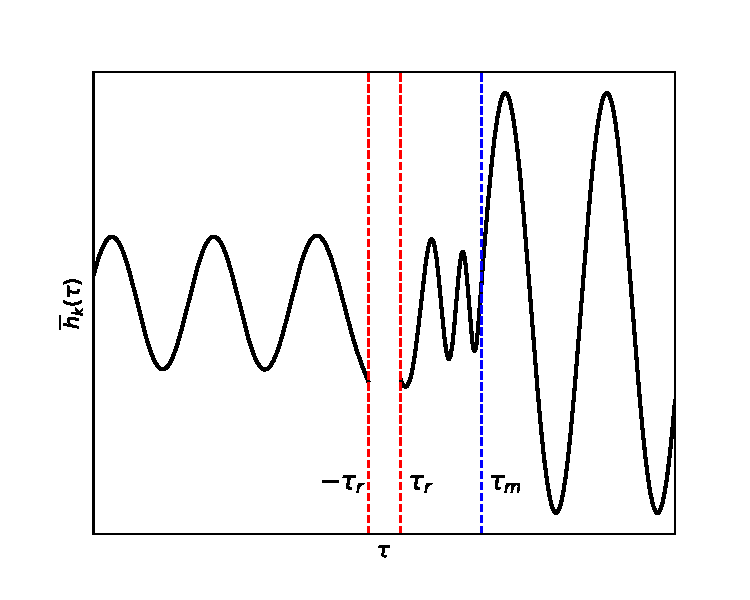
\includegraphics[scale=0.65]{fig/fig1.pdf}
    \caption{Evolution of the real part of $\overline{h}_k(\tau)$. There is a gap in the domain of the conformal time from $-\tau_r$ to $\tau_r$, but $\overline{h}_k(\tau)$ and $\overline{h}_k'(\tau)$ remain continuous. This is a numerical solution to Eq.\ \ref{eqn:eom}, and the exact values for the parameters are detailed in the code \cite{GH}.}
    \label{fig:mode}
\end{figure}

We consider graviton masses on the order of the Hubble scale, and so the evolution of the GWs during inflation will be important.
The scale factor, as described in Eq.\ (4) of Ref.\ \cite{Fujita:2018ehq}, is
\begin{equation}\label{eqn:scale_fac}
    a(\tau) = 
    \begin{cases}
        -1/(H_{\inf}\tau) & \tau < \tau_r \\
        a_r \tau/\tau_r & \tau > \tau_r \\
   \end{cases} \ ,
\end{equation}
where $H_{\inf}$ is the Hubble parameter during inflation when the scale corresponding to the Cosmic Microwave Background exits the Hubble horizon and $a_r$ is the scale factor at the reheating time $\tau_r = 1/(a_r H_{\inf})$. We will assume $a_r$ is fixed in this discussion, while $H_{\inf}$ and $\tau_r$ may vary. The bounds on $H_{\inf}$ are discussed in Ref.\ \cite{Jiang:2015qor}, and they will be respected in this paper. The scale factor in this model has a peculiar behavior where it is not defined in the region $(-\tau_r, \tau_r)$ and only takes values outside of that interval. This is to allow for the scale factor and its first derivative to be continuous and to avoid the singularity at $\tau = 0$. % perhaps expalin more about this weird behavior of the conformal time during inflation 
Fig.\ \ref{fig:mode} illustrates how a generic mode function would look like, showing  the discontinuity in the conformal time. The behavior in the three regions of $\tau$ are discussed in detail in Ref.\ \cite{Fujita:2018ehq}.
We will use the mass function from Eq.\ 5 of Ref.\ \cite{Fujita:2018ehq}
\begin{equation}\label{eqn:mass_case}
    M_\text{GW}(\tau) = 
    \begin{cases}
        m & \tau < \tau_m \\
        0 & \tau > \tau_m
   \end{cases} \ ,
\end{equation} 
where $\tau_m$ is some conformal time during the radiation dominated era when the mass instantaneously drops to 0. For more discussion about why the time is chosen to be in the radiation dominated era, refer to Footnote 2 of Ref.\ \cite{Fujita:2018ehq}. 

\section{Energy Density of gravitational waves}\label{sec:energy}
When we study models of gravitation, we often want to know how sub-horizon GWs from the primordial era are influenced. The energy density spectrum of these GWs at the present time as a function of frequency is perhaps the most practical way to observe the effects of beyond-GR theories. We want to look at the energy fraction of the GWs per logarithmic interval of k at the current time. We have the following definition for the energy density 
\begin{equation}\label{eqn:omega_sfm}
    \Omega_\text{GW} = \frac{1}{\rho_c}\frac{d \rho_\text{GW}} {d \log{k}} \ ,
\end{equation}
where $\rho_c = 3H^2/8\pi G$ is the critical density, and we note that the derivative with respect to $\log k$ is a notational way of representing the spectral density of $\rho_\text{GW}$ (see Footnote 65 of Ref.\ \cite{Maggiore:v1}). Our energy density today is defined in terms of the primordial tensor power spectrum $\mathcal{P}_0(f)$ as detailed in Eq.\ 19.288 of Ref.\ \cite{Maggiore:v2}
\begin{equation}\label{eqn:omega_0_sfm}
    \Omega_{\text{GW},0}(f) = \frac{\pi^2}{3a_0^2H_0^2}f^2 \mathcal{P}_0(f) \ , 
\end{equation}
where $a_0 = a(\tau_0) = 1$. We will find the power spectrum in MG by finding the form of the enhancement factor that will amplify the GR power spectrum.  

We take the power spectrum from Eq.\ 14 of Ref.\ \cite{Fujita:2018ehq}
\begin{equation}\label{eqn:p_sfm}
    \mathcal{P}(\tau, k) \sim \frac{\tau_m}{\tau_r}(k\tau_r)^{3-2\nu}\mathcal{P}_{\text{GR}}(\tau,k)\ , 
\end{equation}
where $\mathcal{P}_{\text{GR}}$ is the power spectrum of the massless tensor modes from inflation, and $\nu$ is defined by 
\begin{equation}\label{eqn:nu}
    \nu = \sqrt{\frac{9}{4} - \frac{m^2}{H_{\inf}^2}}\ .
\end{equation}
This expression for the power spectrum is found by solving the equation of motion for the mode function and finding the expression for $\overline{h}_k$ deep in the massless phase (see Sec.\ III(iii) of Ref.\ \cite{Fujita:2018ehq} for more details). As for the GR power spectrum, we can approximate it by using the transfer function detailed in Ref.\ \cite{Kuroyanagi:2014nba}. To briefly recount, the power spectrum in the GR case is 
\begin{equation}\label{eqn:p_gr_sfm}
    \mathcal{P}_{\text{GR}} = \mathcal{P}^{\text{prim}}_{T} T^2_T(k) \ ,
\end{equation}
where $\mathcal{P}^{\text{prim}}_{T}$ is the primordial tensor power spectrum 
and $T_{T}$ is the transfer function describing the standard reheating scenario in which the universe had a short matter-dominated era after inflation before reheating ended. $\mathcal{P}^{\text{prim}}_{T}$ is defined in Eq.\ 7 of Ref.\ \cite{Kuroyanagi:2014nba} as follows
\begin{equation}\label{eqn:pt}
    \mathcal{P}_{T}^{\text{prim}}(k) = A_T(k_{\text{ref}})\left(\frac{k}{k_{\text{ref}}}\right)^{n_T} \ ,
\end{equation}
where $A_T(k_{\text{ref}})$ is the amplitude at the reference scale,
\hspace{-1em}measured to be precisely $4.4\times 10^{10}$, and $n_T$ is the spectral index. The reference scale $k_{\text{ref}}$ is chosen to be 0.01 Mpc$\/^{-1}$. $T_{T}$ is defined in Eq.\ 12 of Ref.\ \cite{Kuroyanagi:2014nba} in the following way
\begin{equation}\label{eqn:tt}
    T_T^2(k) = \Omega_m^2 \frac{g_*(T_\text{in})}{g_{*0}} \frac{g_{*s0}^{4/3}}{g_{*s}^{4/3}(T_{\text{in}})} \frac{9j_1^2(k\tau_0)}{(k\tau_0)^2}T_1^2(x_{\text{eq}}) T_2^2(x_R) \ ,
\end{equation}
where $g_{*}(T_\text{in})$ and $g_{*0}$ are the relativistic degrees of freedom at the inflation temperature scale and the present respectively, $g_{*s}(T_\text{in})$ and $g_{*s0}$ are their counterparts for entropy, $j_1(k\tau_0)$ is the 1st spherical Bessel function whose approximation $j_1(k\tau_0) \simeq 1/(\sqrt{2}k\tau_0)$ will be used, the fitting functions are empirically found to be $T_1^2(x) = 1+1.57x+3.42x^2$ and $T_2^2(x) = (1-0.22x^{1.5} + 0.65x^2)^{-1}$, and $x_i \equiv k/k_i$. The values for all of the constants and the forms of the functions are taken from Sec. 2.1 of Ref.\ \cite{Kuroyanagi:2014nba}. 
Since we are interested in the energy density at the present, we consider $\Omega_{\text{GW},0}(f) = \Omega_\text{GW}(\tau_0,f)$
\begin{equation}\label{eqn:om_gw_0}
    \Omega_{\text{GW},0}(f) = \frac{\pi^2f^2}{3a_0^2 H_0^2}\frac{\tau_m}{\tau_r}(k\tau_r)^{3-2\nu}\mathcal{P}_{\text{GR}}(k) \ .
\end{equation}
In anticipation of our consideration of certain parameters in the next section, we look at the behavior of the energy density as a function of different parameters. Fig.\ \ref{fig:contours} shows how $\Omega_{\text{GW},0}$ varies with changing $f$ and $M_\text{GW}, \tau_m$, and $H_{\inf}$. We note that in Fig.\ \ref{fig:contours} for the topmost and bottommost plots where we are not varying the ratio $\tau_m/\tau_r$, but for the bottom subplot, we are varying it indirectly since $\tau_r$ changes with $H_{\inf}$.

To comment on the shape of the energy density predicted inflationary theory, we note that there is a change in the slope in the low frequency range, visible near $10^{-17}$ Hz in Fig.\ \ref{fig:contours} and more clearly Fig.\ \ref{fig:supp}. This can be explained by the fact that modes with a sufficiently low frequency have not entered the cosmological horizon. The equation of motion from Eq.\ \ref{eqn:eom} allows for a growing solution of $\overline{h}_k \propto a$ \cite{Gumrukcuoglu:2012wt}. This causes the energy density to grow as the frequency of the mode becomes lower past the point of horizon reentry. 

\section{Results}\label{sec:results}
We now discuss the region of the parameter space that can potentially explain the signals from NG15. The constraints we can place on the SFM model based on NG15 are done by seeing how we can change the parameters $M_{\text{GW}}, H_{\inf},$ and $\tau_m$ to fit the signal. Our initial approach of fixing $H_{\inf}$ to $10^8 \GeV$, like in Ref.\ \cite{Fujita:2018ehq} and letting $m$ and $\tau_m$ vary didn't produce any gravitational wave energy density from inflation that could possibly reproduce NG15. We see in the middle plot of Fig.\ \ref{fig:contours} that increasing $\tau_m$ uniformly increases the primordial energy density. 

\begin{figure}
\begin{subfigure}{.5\textwidth}
  \centering
  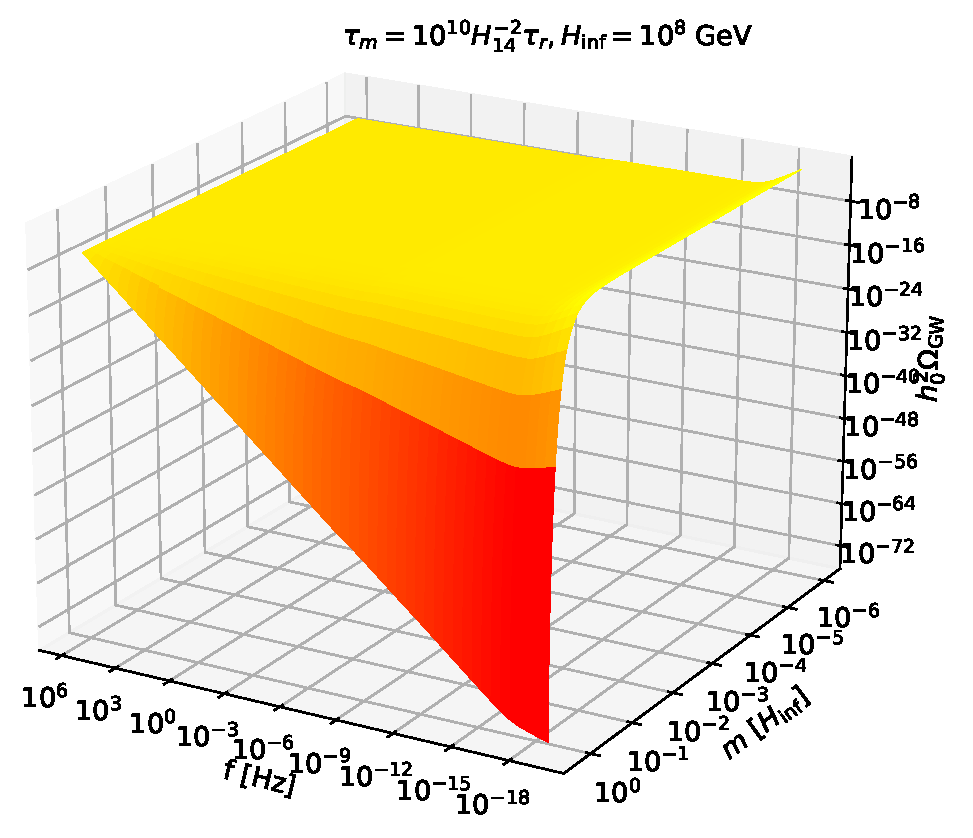
\includegraphics[width=.88\linewidth]{fig/fig2a.pdf}  
  \label{fig:contour-a}
\end{subfigure}
\begin{subfigure}{.5\textwidth}
  \centering
  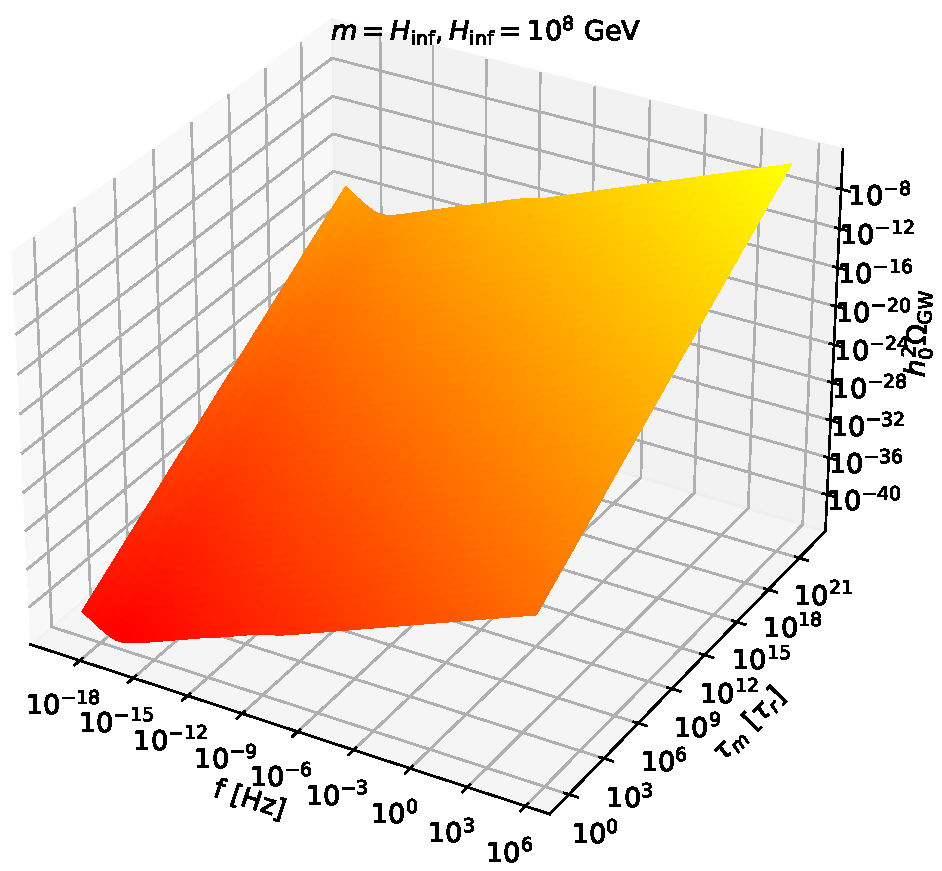
\includegraphics[width=.88\linewidth]{fig/fig2b.pdf}  
  \label{fig:contour-b}
\end{subfigure}
\begin{subfigure}{.5\textwidth}
  \centering
  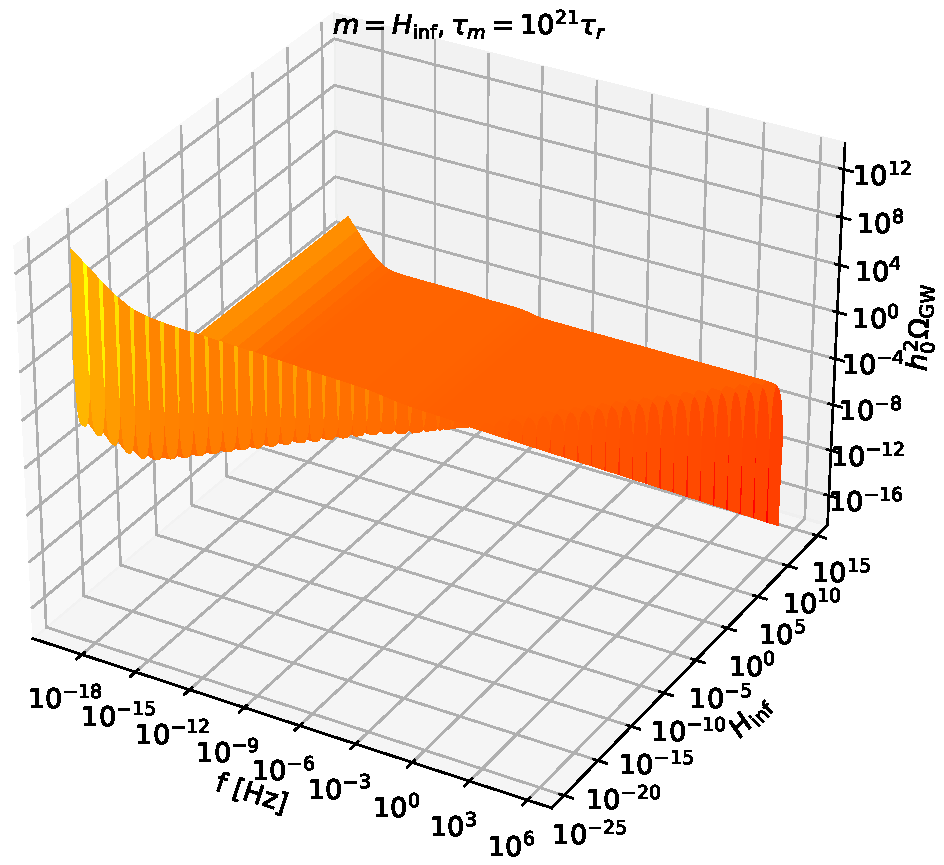
\includegraphics[width=.88\linewidth]{fig/fig2c.pdf}  
  \label{fig:contour-c}
\end{subfigure}
\caption{We plot $\Omega_{\text{GW},0}$ as a function of $f$ and $m$ (top), $\tau_m$ (middle), and $H_{\inf}$ (bottom). The frequency ranges from the scale corresponding to matter-radiation inequality ($\sim 3\times10^{-16}$ Hz) to the inflationary UV cutoff ($\sim 1/(2\pi\tau_r)$ \cite{Fujita:2018ehq}).} 
\label{fig:contours}
\end{figure}

\begin{figure*}
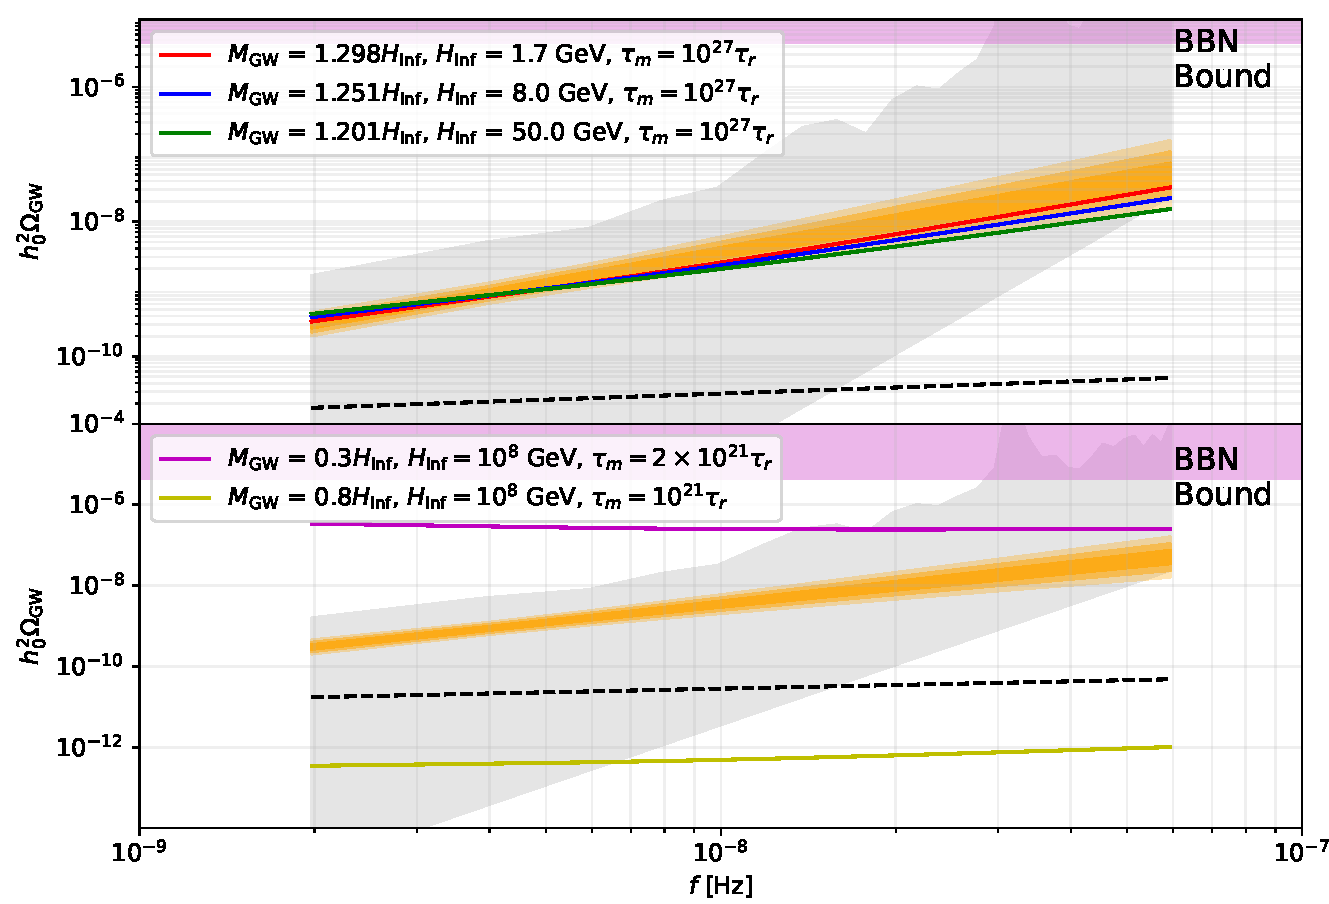
\includegraphics[width=\textwidth]{fig/fig3.pdf} 
\caption{GWB produced by the SFM model. Both figures: we show the BBN excluded region shaded in purple at the top, the periodogram for a Hellings-Down-correlated free spectral process \cite{Agazie:2023} in shaded grey, the $1\sigma$, $2\sigma$, and $3\sigma$ posterior medians for NG15 \cite{Agazie:2023} in darker to lighter orange respectively, and the GWB spectrum produced by an astrophysical population of inspiraling SMBHBs with parameters detailed in Eq.\ A1 of Ref.\ \cite{Afzal:2023} as a black dotted line. Top: The red curve is the GWB spectra fitted to the $1\sigma$ posterior, the blue curve is fitted to the $2\sigma$ posterior, and the green curve is fitted to the $3\sigma$ posterior. Bottom: the purple curve is the energy density that respects the BBN bound for high frequency and passes through the upper limit of the free spectral process of the data, and the golden curve is the energy density that respects the CMB bound for low frequency and passes through the lower limit of the free spectral process of the data.} 
\label{fig:GWB}
\end{figure*}

By varying the other two parameters, $M_{\text{GW}}$ and $H_{\inf}$, we found resulting energy densities that lie within $1\sigma$, $2\sigma$, and $3\sigma$ of the power law posterior of the signal. Our values for the parameters were $M_{\text{GW}} = 1.298H_{\inf}$ and $H_{\inf} =  1.7 \GeV$ to stay within $1\sigma$ of the posterior, $M_{\text{GW}} = 1.251H_{\inf}$ and $H_{\inf} = 8.0 \GeV$ to stay within $2\sigma$ of the posterior $M_{\text{GW}} = 1.201H_{\inf}$ and $H_{\inf} = 50.0 \GeV$ to stay within $3\sigma$ of the posterior. We have kept the ratio $\tau_m/\tau_r$ constant for these three energy densities, although the magnitude of $\tau_m$ changes due to the change in $\tau_r$. 

The bound on $\Omega_{GW,0}$ made from the big bang nucleosynthesis (BBN) limits comes from the explicit limit on the integral of the energy density (Eq.\ 3.3 of Ref.\ \cite{Tanin:2020qjw}) 
\begin{equation} \label{eqn:bbn_int}
    \int_{f = f_{BBN}}^{f = \infty}\mbox{d}(\ln{f}) h_0^2\Omega_{GW,0}(f) \lesssim 1\times 10^{-6} \ ,
\end{equation} 
where $f_{BBN}$ is the present day frequency at which the gravitational waves at the time of BBN were inside the horizon and therefore contribute to the expansion of the Universe and is approximately $1.5\times 10^{-11}$ Hz (Eq.\ 22.290 of Ref.\ \cite{Maggiore:v2}). We can reformulate Eq.\ \eq{eqn:bbn_int} as a bound on the energy density rather than the integral of the energy density, since in most cosmological mechanisms, including the one we consider in this paper, the spectrum covers at least one decade of frequency. So thus we have the bound 
\begin{equation}
    \Omega_{\text{GW}}(f) \lesssim 1 \times 10^{-6},\ f > f_{\text{BBN}} \ .
\end{equation}

Although it may appear that the energy densities we consider in Fig.\ \ref{fig:GWB} violate the BBN bound for higher frequencies, since the energy densities in the full range of frequencies pass into the forbidden energy range as we see in Fig.\ \ref{fig:supp}, we keep in mind that the BBN bound only applies to gravitational waves that were blue tilted by massive gravitons before BBN took place. If the graviton were massive during BBN 
\begin{equation}\label{eqn:massive_bbn}
    \frac{\tau_m}{\tau_r} \gtrsim \frac{\tau_{\text{BBN}}}{\tau_r} = \sqrt{\frac{H_{\inf}}{H_{\text{BBN}}}}\ ,
\end{equation}
then we should be able to relax the BBN bound. This is because gravitons do not contribute to the relativistic degrees of freedom during BBN \cite{Fujita:2018ehq}, since they would have had a significant mass, meaning that they contribute to non-relativistic species.

We note that if we still wish to conservatively respect the BBN bound in the same way as Ref.\ \cite{Fujita:2018ehq} and still have our theory of MG be consistent with NG15, we can use the parameters investigated by Ref.\ \cite{Fujita:2018ehq} with some slight modifications. We see that to order to partially produce the signal in the higher energy density and frequency regime, as shown by the purple curve in Figs.\ \ref{fig:GWB} and \ref{fig:supp}, the CMB bound must be violated. On the other hand, we find that while attempting to partially produce the signal in the lower energy density and frequency regime, as shown by the golden curve in Figs.\ \ref{fig:GWB} and \ref{fig:supp}, the SMBHB power spectrum turns out to be a better fit to the signal. The requirement to respect both bounds to reproduce the signal seems to be mutually exclusive. But if we do not conservatively respect the BBN bound, then it appears that we can achieve good agreement with the signal, with the caveat being that the cutoff time for the graviton mass is deep into the matter dominated era.

\begin{figure}[ht]
    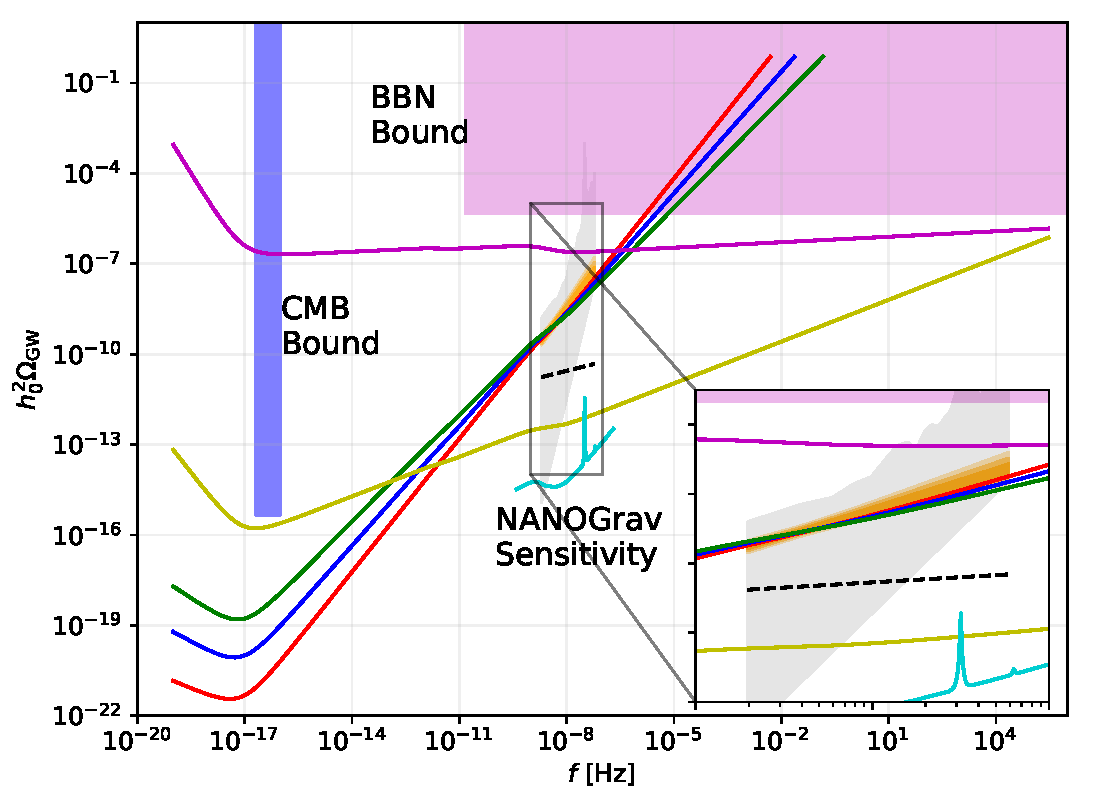
\includegraphics[width=\linewidth]{fig/fig4.pdf}
    \caption{The energy densities in Fig.\ \ref{fig:GWB} plotted over the frequency range specified in Fig.\ \ref{fig:contours}. The red, blue, green, purple, and golden curves correspond to the energy densities of the same color in Fig.\ \ref{fig:GWB}. The turquoise curve below the energy densities is the sensitivity curve for NG15. The blue shaded region on the left is the excluded region from the CMB bound. The BBN bound region may be ignored if the graviton remains massive during BBN.} 
    \label{fig:supp}
\end{figure}

\section{Discussion}\label{sec:discussion}
In this paper, we discussed how the constant mass and step function mass models of massive gravity can be constrained by the 15-year NANOGrav data set. We note that the selection of the parameters in the step function mass model leads to energy densities that violate the BBN bound for higher frequencies, specifically in the region of frequencies $\gtrsim 10^{-6}$ Hz. We propose that there could be some mechanism that suppresses the energy density of gravitational waves from the primordial era for those frequencies. A mechanism analogous to the damping of the energy density from the free-streaming neutrinos \cite{Durrer:1997ta,Weinberg:2003ur} could be behind such a suppression necessary to obey the BBN bound, if this model of MG is to be the dominant source of the background. For example, the propagation of gravitational waves in the turbulent primordial radiation-dominated plasma\footnote{Turbulent sources induce GWs through their anisotropic stress tensor, with $\Omega_{\rm GW} \propto f^{-8/3}$ for  high frequencies.} \cite{RoperPol:2019wvy} may provide the necessary suppression at the short wavelength regime \cite{Deryagin:1986}. 

Observations of gravitational waves have mostly ruled out the possibility of gravitons with a very low but nonzero mass, since the expectation that a peak, which is predicted from such a model \cite{Gumrukcuoglu:2012wt}, could be present for lower frequencies is becoming slim. Therefore, the more plausible possibility of massive gravity is the scenario in which the graviton mass is a non-constant function of time. We have only considered a step function as the time dependent function, but more complicated functions are possible. The mechanism behind such a mass decay would come from the exact nature of the phase transition of the gravitational field. It may be fruitful to pursue an investigation to place constraints on the specific evolution of the mass during the phase transition. Then, we would be able to probe the mass evolution and shed insight into the time dependent behavior beyond a step function. 

Additionally, further observations that place constraints on the Hubble rate of expansion, the scale factor, and the time associated with inflation would be able to constrain the parameters of this theory. In addition to signals we have already observed with interferometers, we expect a more drastic suppression for higher frequencies than we discuss. Future work may investigate the nature of this suppression and propose plausible mechanisms for it.

\vspace{2mm}
{\bf Data availability}---The NANOGrav 15-Year data used in this paper is available at \href{https://nanograv.org/science/data}{NANOGrav}. Source code to reproduce all of the figures in this paper is available in our GitHub repository \cite{Choi_constrain_mass_nanograv_15}. 

\vspace{2mm}
{\bf Acknowledgements}--- We thank Sachiko Kuroyanagi and Shinji Mukohyama for helpful discussions related to the model \cite{Fujita:2018ehq} and feedback. We appreciate discussions and useful comments from Axel Brandenburg, Neil J.\ Cornish, Arthur B.\ Kosowsky, and Sayan Mandal. We thank Emma Clarke, Jeffrey S.\ Hazboun, and William G.\ Lamb for their help with plotting the NANOGrav data. We thank the organizers and participants of the PITT PACC workshop ``Unravelling the Universe with Pulsar Timing Arrays Workshop" during which the paper has been finalized. TK and MG acknowledge partial support from the NASA Astrophysics Theory Program Award 80NSSC22K0825.

\bibliographystyle{apsrev4-2_edited}
\bibliography{refs}

\clearpage
\end{document}